\documentclass{exam}
\usepackage{amsmath}
\usepackage{nicematrix}
\usepackage{extpfeil}
\usepackage{amsthm}
\usepackage{gensymb}
\usepackage{amsfonts}
\usepackage{tikz}
\usepackage{pgfplots}
\usepackage{array}
\usepackage{hyperref}
\usepackage{nameref}
\usepackage[x11names]{xcolor}
\usepackage[most]{tcolorbox}

\pgfplotsset{compat=1.18}
\printanswers

\newcommand{\ZZ}{\mathbb Z}
\newcommand{\QQ}{\mathbb Q}
\newcommand{\NN}{\mathbb N}
\newcommand{\RR}{\mathbb R}
\newcommand{\braces}[1]{\ensuremath{\left\{#1 \right\}}}
\newcommand{\Span}[1]{\ensuremath\text{Span}\braces{#1}}
\newcommand{\ee}{\mathbf{e}}

\hypersetup{colorlinks=true, linktoc=section, linkcolor=blue}

\pagestyle{headandfoot}
\firstpageheadrule
\runningheadrule
\firstpageheader{Prof. Shtelen \\ Linear Algebra}{Homework 2}{Jeevan Shah}
\runningheader{Linear Algebra \\ Homework 2}{}{Shah}
\firstpagefooter{}{}{}
\runningfooter{ }{\thepage}{ }

\printanswers

\newenvironment{amatrix}[1]{%
  \left(\begin{array}{@{}*{#1}{c}|c@{}}
}{%
  \end{array}\right)
}

\begin{document}
\underline{\#29 [1.7]:} Describe the possible echelon forms of the matrix $A$ such that $A$ is a $3 \times 3$ matrix with linearly independent columns
\begin{solution}
    \[
        \boxed{
            \begin{pmatrix}
                \blacksquare & * & * \\
                0 & \blacksquare & * \\
                0 & 0 & \blacksquare
            \end{pmatrix}
        }
    \]
    Where $\blacksquare\in\RR \setminus {0}$, $* \in \RR$ and $0=0$. This is the only possible echelon form for $A$ since in order for the columns to be linearly independent the system $A\vec{x}=\vec{0}$ must only have the trivial solution. This will occur when each column in $A$ contains a pivot.
\end{solution}

\underline{\#37 [1.7]:} Given the matrix $A$ below, observe that the third column is the sum of the first two columns. Find a nontrivial solution of $A\vec{x}=\vec{0}$ \textbf{without using row operations}
\[
    A = \begin{pmatrix}
        2 & 3 & 5 \\
        -5 & 1 & -4 \\
        -3 & -1 & -4 \\
        1 & 0 & 1
    \end{pmatrix}
\]
\begin{solution}
    Start by noticing that
    \[
        A\vec{x} = \vec{0} \Leftrightarrow 
        x_1\begin{pmatrix}
            2 \\ -5 \\ -3 \\ 1
        \end{pmatrix}
        + 
        x_2\begin{pmatrix}
            3 \\ 1 \\ -1 \\ 0
        \end{pmatrix}
        + 
        x_3\begin{pmatrix}
            5 \\ -4 \\ -4 \\ 1
        \end{pmatrix}
        = \vec{0}
    \]
    Now, for any given row in $A$, the third column is the sum of the first two columns. Thus
    \[
        \boxed{\vec{x} = \begin{pmatrix} 1 \\ 1 \\ -1\end{pmatrix}} \Rightarrow A\vec{x} = \vec{0}
    \]
\end{solution}

\underline{\#11 [1.8]:} Let $\vec{b}$ and $A$ be the matricies below. Is $\vec{b}$ in the range of the linear transformation $\vec{x}\mapsto\,A\vec{x}$? Why or why not?
\[
    A = \begin{pmatrix}
        1 & -4 & 7 & -5 \\
        0 & 1 & -4 & 3 \\
        2 & -6 & 6 & -4
    \end{pmatrix}
    \text{ and }
    \vec{b} = \begin{pmatrix}
        -1 \\ 1 \\ 0
    \end{pmatrix}
\]
\begin{solution}
    Consider the augmented matrix $(A | B)$:
    \begin{align*}
        \begin{amatrix}{4}
        1 & -4 & 7 & -5 & -1 \\
        0 & 1 & -4 & 3 & 1 \\
        2 & -6 & 6 & -4 & 0
        \end{amatrix}
        &\xrightarrow{R_3 \to R_3 - 2R_1}
        \begin{amatrix}{4}
        1 & -4 & 7 & -5 & -1 \\
        0 & 1 & -4 & 3 & 1 \\
        0 & 2 & 8 & 6 & 2
        \end{amatrix}\\
        &\xrightarrow{R_3 \to R_3 - 2R_2}
        \begin{amatrix}{4}
        1 & -4 & 7 & -5 & -1 \\
        0 & 1 & -4 & 3 & 1 \\
        0 & 0 & 0 & 0 & 0
        \end{amatrix}
    \end{align*}
    $\therefore$ no pivots in the final column implies that the system $A\vec{x}=\vec{b}$ is consistent so $\vec{b} \in \mathcal{T}^{\text{img}}$ where $\mathcal{T}$ is the linear transformation given by the map $\vec{x}\mapsto\,A\vec{x}$
\end{solution}


\underline{\#31 [1.8]:} Let $\mathcal{T}: \RR^{2} \to \RR^{2}$ be the linear transformation that reflects each point through the $x_1$-axis. Make two sketches that illustrate the two main properties of linear transformations.
\begin{solution}
    See the below figures: \\
    \begin{minipage}{0.45\linewidth}
        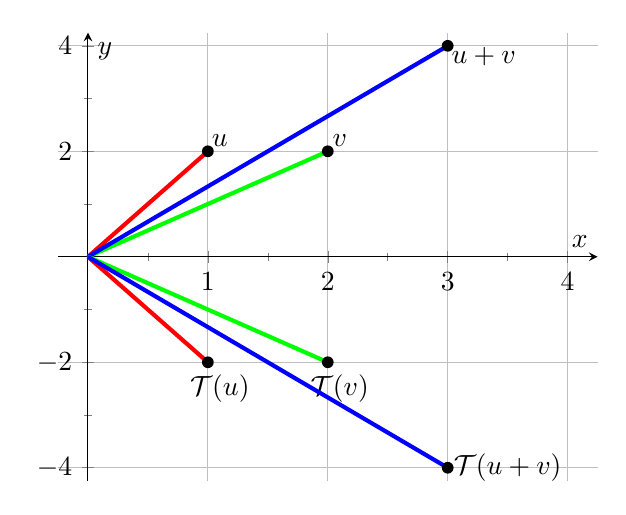
\begin{tikzpicture}
            \begin{axis}[
                grid = major,
                axis lines = center,
                xmin = -0.25,
                xmax = 4.25,
                ymin = -4.25,
                minor tick num = 1,
                ymax = 4.25,
                % xticklabels = {},
                % yticklabels = {},
                xlabel = {$x$},
                ylabel = {$y$},
            ]

            \draw[line width=1.5pt, red] (axis cs: 0, 0) -- (axis cs: 1, 2);
            \node[circle, fill, inner sep=1.5pt] (A) at (axis cs: 1, 2) {};
            \node[] (A) at (axis cs: 1.1, 2.2) {$u$};

            \draw[line width=1.5pt, green] (axis cs: 0, 0) -- (axis cs: 2, 2);
            \node[circle, fill, inner sep=1.5pt] (A) at (axis cs: 2, 2) {};
            \node[] (A) at (axis cs: 2.1, 2.2) {$v$};

            \draw[line width=1.5pt, blue] (axis cs: 0, 0) -- (axis cs: 3, 4);
            \node[circle, fill, inner sep=1.5pt] (A) at (axis cs: 3, 4) {};
            \node[] (A) at (axis cs: 3.3, 3.8) {$u + v$};

            \draw[line width=1.5pt, red] (axis cs: 0, 0) -- (axis cs: 1, -2);
            \node[circle, fill, inner sep=1.5pt] (A) at (axis cs: 1, -2) {};
            \node[] (A) at (axis cs: 1.1, -2.5) {$\mathcal{T}(u)$};

            \draw[line width=1.5pt, green] (axis cs: 0, 0) -- (axis cs: 2, -2);
            \node[circle, fill, inner sep=1.5pt] (A) at (axis cs: 2, -2) {};
            \node[] (A) at (axis cs: 2.1, -2.5) {$\mathcal{T}(v)$};

            \draw[line width=1.5pt, blue] (axis cs: 0, 0) -- (axis cs: 3, -4);
            \node[circle, fill, inner sep=1.5pt] (A) at (axis cs: 3, -4) {};
            \node[] (A) at (axis cs: 3.5, -4) {$\mathcal{T}(u + v)$};

            \end{axis}
        \end{tikzpicture}
    \end{minipage}
    \hfill
    \begin{minipage}{0.45\linewidth}
        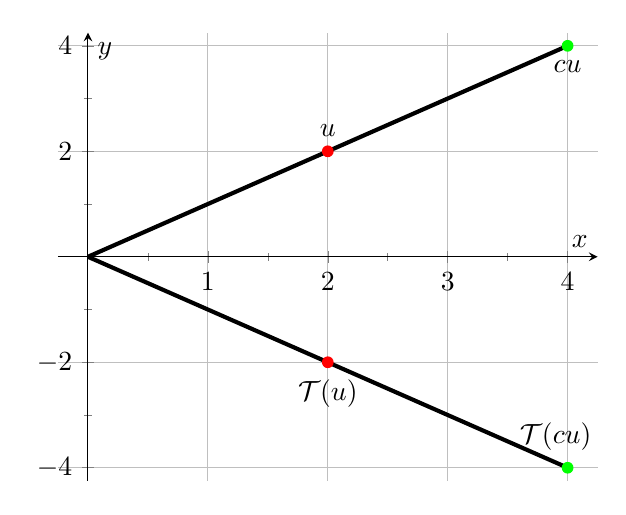
\begin{tikzpicture}
            \begin{axis}[
                grid = major,
                axis lines = center,
                xmin = -0.25,
                xmax = 4.25,
                ymin = -4.25,
                minor tick num = 1,
                ymax = 4.25,
                % xticklabels = {},
                % yticklabels = {},
                xlabel = {$x$},
                ylabel = {$y$},
            ]

            \draw[line width=1.5pt] (axis cs: 0, 0) -- (axis cs: 4, 4);
            
            \node[circle, fill, inner sep=1.5pt, red] (A) at (axis cs: 2, 2) {};
            \node[] (A) at (axis cs: 2, 2.4) {$u$};

            \node[circle, fill, inner sep=1.5pt, green] (A) at (axis cs: 4, 4) {};
            \node[] (A) at (axis cs: 4, 3.6) {$cu$};

            \draw[line width=1.5pt] (axis cs: 0, 0) -- (axis cs: 4, -4);

            \node[circle, fill, inner sep=1.5pt, red] (A) at (axis cs: 2, -2) {};
            \node[] (A) at (axis cs: 2, -2.6) {$\mathcal{T}(u)$};

            \node[circle, fill, inner sep=1.5pt, green] (A) at (axis cs: 4, -4) {};
            \node[] (A) at (axis cs: 3.9, -3.4) {$\mathcal{T}(cu)$};
            \end{axis}
        \end{tikzpicture}
    \end{minipage}
\end{solution}

\underline{\#15 [1.9]:} Fill in the missing entries of the matrix, assuming that the equation holds for all values of the variables.
\[
    \begin{pmatrix}
        ? & ? & ? \\
        ? & ? & ? \\
        ? & ? & ? 
    \end{pmatrix}
    \begin{pmatrix}
        x_1 \\ x_2 \\ x_3
    \end{pmatrix}
    = 
    \begin{pmatrix}
        2x_1 - 3x_3 \\
        4x_1 \\
        x_1 - x_2 + x_3
    \end{pmatrix}
\]
\begin{solution}
    Recall that any linear transformation can be put in the from $\mathcal{T}\left(\vec{x}\right) = A\vec{x}$ where $A$ is the matrix with column vectors $\mathcal{T}\left(\textbf{e}_1\right) \dots \mathcal{T}\left(\textbf{e}_n\right)$. Thus, 
    \[
        A = \begin{pmatrix}
            \left(\mathcal{T}\left({\textbf{e}_1}\right)\right) & 
            \left(\mathcal{T}\left({\textbf{e}_2}\right)\right) &
            \left(\mathcal{T}\left({\textbf{e}_3}\right)\right) 
        \end{pmatrix} 
        = 
        \boxed{
            \begin{pmatrix}
                2 & 0 & -3 \\
                4 & 0 & 0 \\
                1 & -1 & 1 
            \end{pmatrix}
        }
    \]
\end{solution}

\underline{\#33 [1.9]:} Determine if the transfromation $\mathcal{T}$ given by the map $\vec{x}\mapsto\,A\vec{x}$, where $A$ is given below, is one-to-one, onto, both, or neither.
\[
    \underset{4 \times 4}{A} = \begin{pmatrix}
        0 & 0 & 0 & 0 \\
        1 & 1 & 0 & 0 \\
        0 & 1 & 1 & 0 \\
        0 & 0 & 1 & 1 
    \end{pmatrix}
\]
\begin{solution}
    Start by moving row 1 to the bottom and shifting the other rows up:
    \[
        A_{\text{REF}} = \begin{pmatrix}
            1 & 1 & 0 & 0 \\
            0 & 1 & 1 & 0 \\
            0 & 0 & 1 & 1 \\
            0 & 0 & 0 & 0 
        \end{pmatrix}
    \]
    Notice that $\text{rank}\left(A_{\text{REF}}\right) \ne 4 \therefore \boxed{\mathcal{T} \text{ is neither one-to-one nor onto.}}$
\end{solution}

\underline{\#7 [2.1]:} If a matrix $A$ is $5 \times 3$ and the product $AB$ is $5 \times 7$, what is the size of $B$?
\begin{solution}
    The number of columns in $A$ must match the number of rows in $B$ so $B$ must have $3$ rows. The number of columns of $B$ must match the number of columns in $AB$ so $B$ must have $7$ columns.\ \fbox{Thus, $B$ is a $3 \times 7$ matrix.}
\end{solution}


\underline{\#25 [2.1]:} If $A$ and $AB$ are the matricies given below, determine the first and second columns of $B$
\[
    A = \begin{pmatrix}
        1 & -2 \\ -2 & 5
    \end{pmatrix}
    \text{ and } 
    AB = \begin{pmatrix}
        -1 & 2 & -1 \\
        6 & -9 & 3
    \end{pmatrix}
\]
\begin{solution}
    Let since $A$ has size $2 \times 2$ and $AB$ has size $2 \times 3$, $B$ must have size $2 \times 3$ as well. Let
    \[B = \begin{pmatrix}
        x_1 & x_3 & * \\ x_2 & x_4 & *
    \end{pmatrix}\]
    Where $*\in\RR$. Then, 
    \[
        AB =  
        \begin{pmatrix}
            1 & -2 \\ -2 & 5
        \end{pmatrix}
        \begin{pmatrix}
            x_1 & x_3 & * \\ x_2 & x_4 & *
        \end{pmatrix}
        =
        \begin{pmatrix}
            -1 & 2 & -1 \\
            6 & -9 & 3
        \end{pmatrix}
    \]
    By definition of matrix multiplication we can find the two systems: \\
    \begin{minipage}{0.47\linewidth}
        \[
            \left.\begin{cases}
                x_1 - 2x_2 &= -1 \\
                -2x_1 + 5x_2 &= 6
            \end{cases}\right] 
            \Rightarrow
            x_2 = 4 \text{ and } x_1 = 7
        \]        
    \end{minipage}
    \hfill
    \begin{minipage}{0.47\linewidth}
        \[
            \left.\begin{cases}
                x_3 - 2x_4 &= 2 \\
                -2x_3 + 5x_4 &= -9
            \end{cases}\right]
            \Rightarrow 
            x_4 = -5 \text{ and } x_3 = -8
        \]
    \end{minipage}
    Thus, 
    \[\boxed{B = \begin{pmatrix}
        7 & -8 & * \\
        4 & -5 & *
    \end{pmatrix}}\]
\end{solution}

\underline{\#7 [2.2]:} Use the inverse of a matrix to solve the system below
\[
    \begin{cases}
        8x_1 + 3x_2 &= 2 \\
        5x_1 + 2x_2 &= 3
    \end{cases}
\]
\begin{solution}
    Consider the system in the from $A\vec{x}=\vec{b}$ where
    \[
        A = \begin{pmatrix}
            8 & 3 \\ 5 & 2
        \end{pmatrix} 
    \]
    Then, $\vec{x}=A^{-1}\vec{b}$ where
    \[
        A^{-1} = \frac{1}{\mathop{\det}A}\begin{pmatrix}
            2 & -5 \\ 
            -3 & 8
        \end{pmatrix} 
        =
        \begin{pmatrix}
            2 & -5 \\
            -3 & 8
        \end{pmatrix}
    \]
    Therefore
    \[
        \vec{x} = A^{-1}\vec{b} = 
        \begin{pmatrix}
            2 & -3 \\
            -5 & 8
        \end{pmatrix}
        \begin{pmatrix}
            2 \\ -1
        \end{pmatrix}
        = 
        \boxed{\begin{pmatrix}
            7 \\ -18
        \end{pmatrix}
        = 
        \begin{pmatrix}
            x_1 \\ x_2
        \end{pmatrix}}
    \]
\end{solution}

\underline{\#43 [2.2]:} Find the inverses of
\[
    \begin{pmatrix}
        1 & 0 & 0 \\
        1 & 1 & 0 \\
        1 & 1 & 1
    \end{pmatrix} 
    \text{ and }
    \begin{pmatrix}
        1 & 0 & 0 & 0 \\
        1 & 1 & 0 & 0 \\
        1 & 1 & 1 & 0 \\
        1 & 1 & 1 & 1 
    \end{pmatrix}
\]
Let $A$ be the corresponding $n\times\,n$ matrix, and let $B$ be its inverse. Guess the form of $B$, and then prove that $AB=I$ and $BA=I$.
\begin{solution}
    Let the first matrix above be $M_1$ and the second $M_2$. We can find the inverse of $M_1$ by augmenting it with $I_3$
    \begin{align*}
        (M_1 | I_3) = \begin{pmatrix}
            1 & 0 & 0 & 1 & 0 & 0 \\
            1 & 1 & 0 & 0 & 1 & 0 \\
            1 & 1 & 1 & 0 & 0 & 1 
        \end{pmatrix}
        \xrightarrow[R_3 \to R_3 - R_1]{R_2 \to R_2 - R_1}
        \begin{pmatrix}
            1 & 0 & 0 & 1 & 0 & 0 \\
            0 & 1 & 0 & -1 & 1 & 0 \\
            0 & 1 & 1 & -1 & 0 & 1 
        \end{pmatrix}
        \xrightarrow{R_3 \to R_3 - R_2}
        \begin{pmatrix}
            1 & 0 & 0 & 1 & 0 & 0 \\
            0 & 1 & 0 & -1 & 1 & 0 \\
            0 & 0 & 1 & 0 & -1 & 1 
        \end{pmatrix}
    \end{align*}
    Thus, 
    \[M_1^{-1} = \begin{pmatrix}
        1 & 0 & 0 \\
        -1 & 1 & 0 \\
        0 & -1 & 1
    \end{pmatrix}\]
    We can follow a similar process for $M_2$ with $I_4$:
    \[
        (M_2 | I_4) = \begin{pmatrix}
            1 & 0 & 0 & 0 & 1 & 0 & 0 & 0 \\
            1 & 1 & 0 & 0 & 0 & 1 & 0 & 0 \\
            1 & 1 & 1 & 0 & 0 & 0 & 1 & 0 \\
            1 & 1 & 1 & 1 & 0 & 0 & 0 & 1
        \end{pmatrix}
        \xrightarrow{\text{ERO}}
        \begin{pmatrix}
            1 & 0 & 0 & 0 & 1 & 0 & 0 & 0 \\
            0 & 1 & 0 & 0 & -1 & 1 & 0 & 0 \\
            0 & 0 & 1 & 0 & 0 & -1 & 1 & 0 \\
            0 & 0 & 0 & 1 & 0 & 0 & -1 & 1 
        \end{pmatrix}
    \]
    Thus, 
    \[
        M_2^{-1} = \begin{pmatrix}
            1 & 0 & 0 & 0 \\ 
            -1 & 1 & 0 & 0 \\
            0 & -1 & 1 & 0 \\
            0 & 0 & -1 & 1
        \end{pmatrix}
    \]
    We can now reasonable guess that for an $n \times n$ matrix $A$ in the corresponding form will have an inverse 
    \[
        A^{-1} = B = \begin{pmatrix}
            1 & 0 & 0 & \cdots & 0 \\
            -1 & 1 & 0 & \cdots & 0 \\
            0 & -1 & 1 & \cdots & 0 \\
            \vdots & \vdots & & \ddots & \vdots \\
            0 & 0 & \cdots & -1 & 1
        \end{pmatrix}
    \]
    Thus, $AB = BA = I_n$.
    \begin{proof}
        We can start with the proof that $AB=I_n$. Begin by noticing that for $1 \leq j \leq n-1$, 
        \[a_j - a_{j+1} = \mathbf{e}_j \text{ and } b_j = \mathbf{e}_j - \mathbf{e}_{j+1}\]
        As well as the fact that $\mathbf{a}_n = \mathbf{b}_n = \mathbf{e}_n$. Now, consider $AB$ in the form 
        \[AB = \begin{pmatrix} A\mathbf{b}_1 & A\mathbf{b}_1 & \cdots & A\mathbf{b}_n \end{pmatrix}\]
        For any $j$ we can see that 
        \[A\mathbf{b}_j = A\left(\mathbf{e}_j - \mathbf{e}_{j+1}\right) = A\mathbf{e}_j - A\mathbf{e}_{j+1} = \mathbf{a}_j - \mathbf{a}_{j+1} = \mathbf{e}_j\]
        Thus, 
        \[AB = \begin{pmatrix} \mathbf{e}_1 & \mathbf{e}_2 & \cdots & \mathbf{e}_n \end{pmatrix} = I_n\]
        It follows that by the uniqueness of inverse matricies that $B = A^{-1}$ therefore by definition of an inverse matrix 
        \[
            AA^{-1} = A^{-1}A = BA = AB = I_n
        \]
    \end{proof}
\end{solution}

\footnotetext{\LaTeX\ code for this document can be found on github \href{https://github.com/jeevanshah07/MATH250/blob/main/homework/homework2/main.tex}{\underline{here}}}
\end{document}